% WebContactsProPlus — sequence: photo upload + resize + thumbnail
\documentclass[border=14pt]{standalone}
\usepackage{tikz}
\usetikzlibrary{positioning, arrows.meta, calc, fit}

\begin{document}
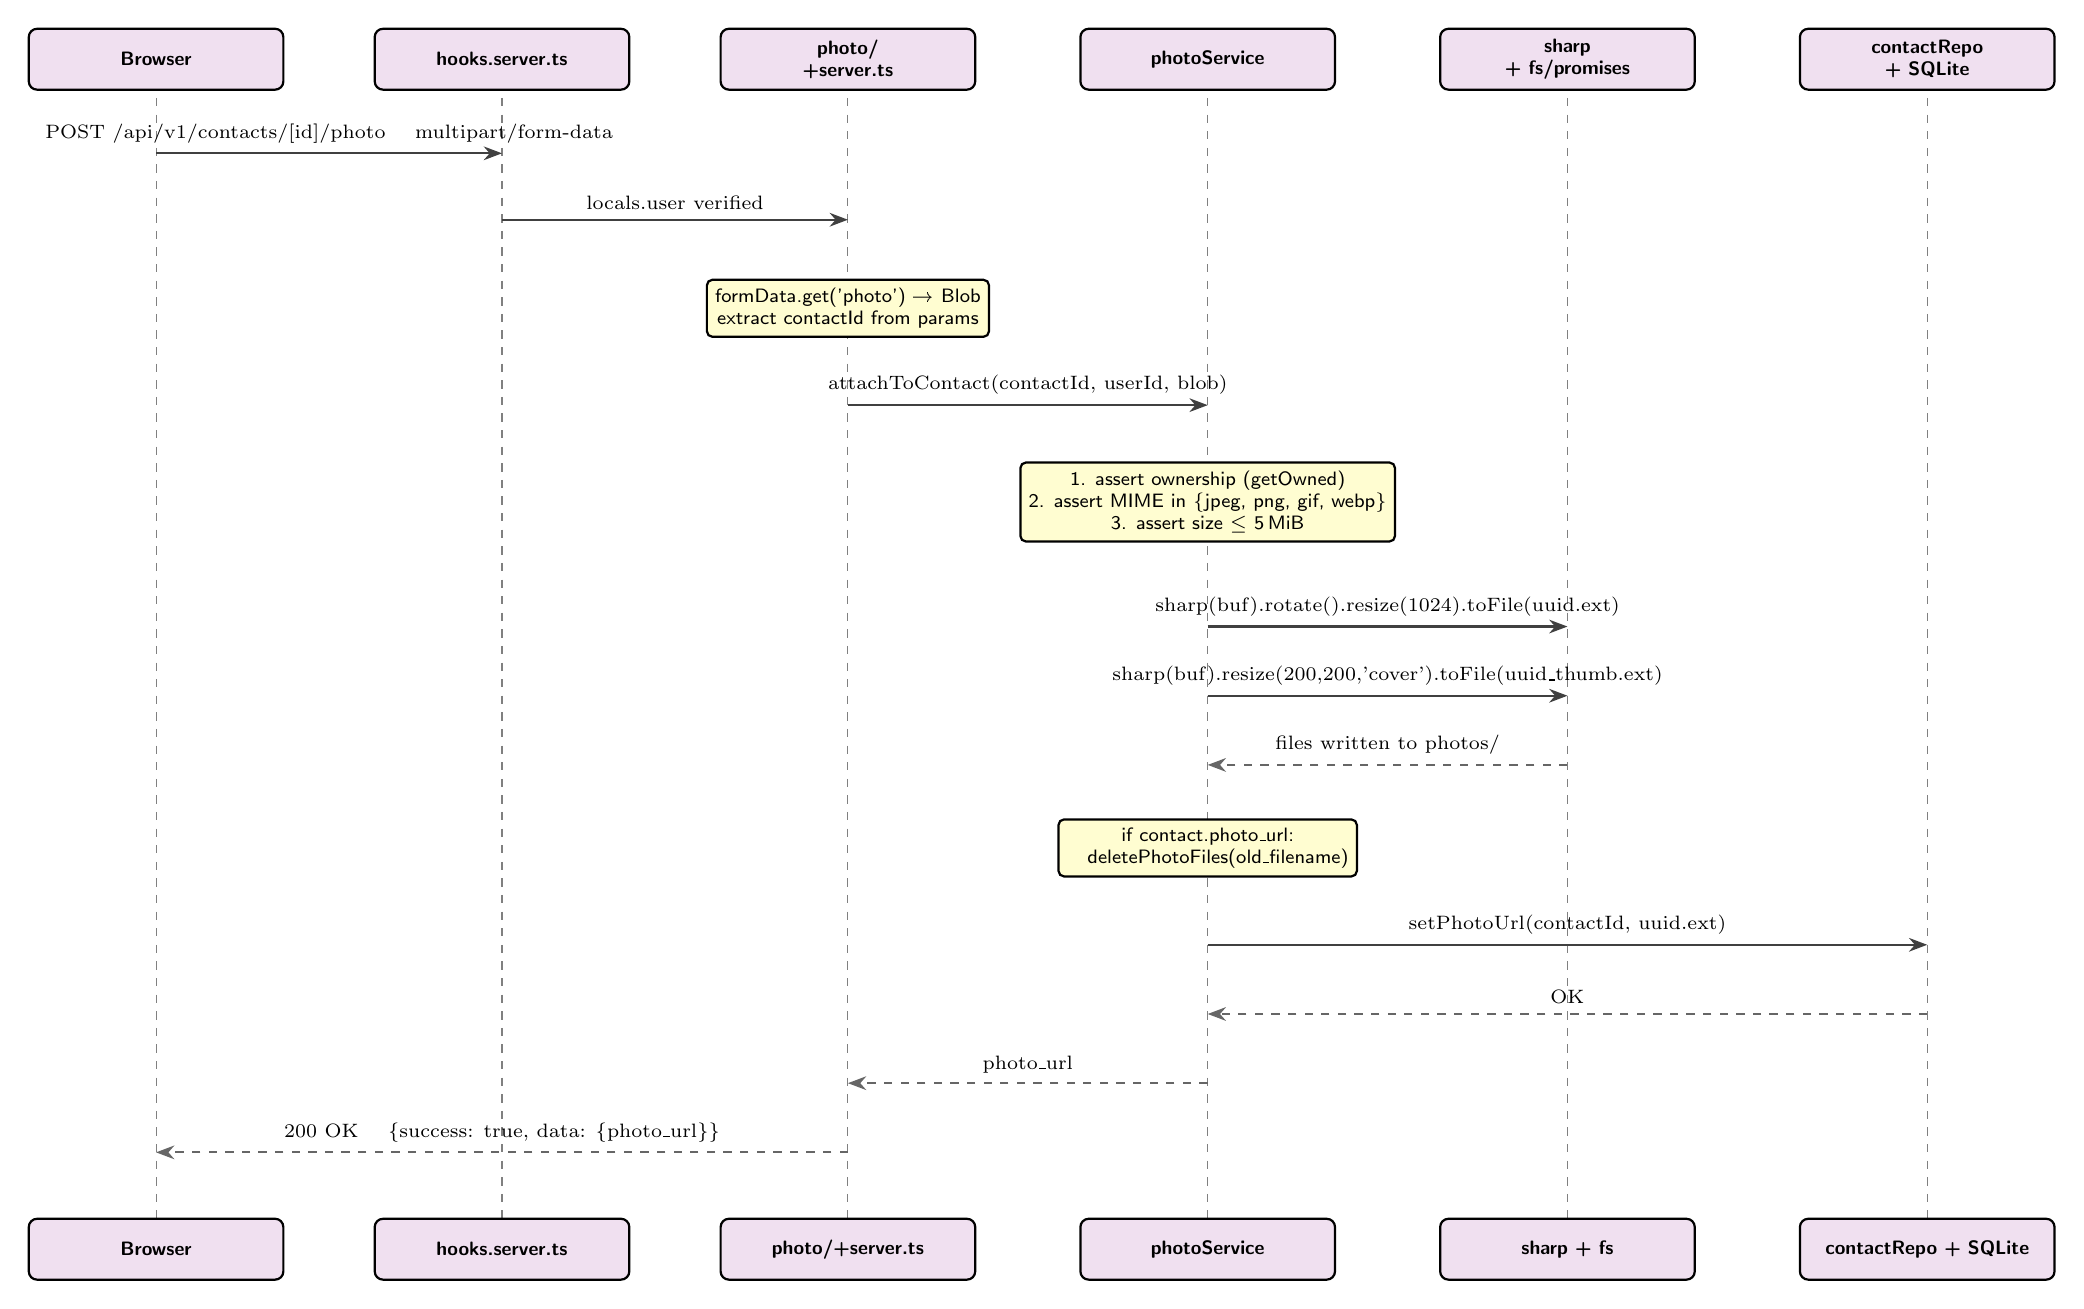
\begin{tikzpicture}[
    >=Stealth,
    font=\sffamily\footnotesize,
    actor/.style={
        draw, thick, fill=violet!12, rounded corners=3pt,
        minimum width=92pt, minimum height=22pt,
        align=center, font=\sffamily\scriptsize\bfseries,
    },
    msg/.style={->, thick, draw=black!75},
    ret/.style={->, thick, draw=black!60, dashed},
    note/.style={
        draw, thick, fill=yellow!18,
        rounded corners=2pt, align=center,
        font=\sffamily\scriptsize, inner sep=3pt,
    },
    lifeline/.style={dashed, draw=black!50},
]

\def\colA{0}
\def\colB{125}
\def\colC{250}
\def\colD{380}
\def\colE{510}
\def\colF{640}

\node[actor] (A) at (\colA pt,0) {Browser};
\node[actor] (B) at (\colB pt,0) {hooks.server.ts};
\node[actor] (C) at (\colC pt,0) {photo/\\+server.ts};
\node[actor] (D) at (\colD pt,0) {photoService};
\node[actor] (E) at (\colE pt,0) {sharp \\ {\scriptsize + fs/promises}};
\node[actor] (F) at (\colF pt,0) {contactRepo \\ {\scriptsize + SQLite}};

\def\bot{-430pt}
\foreach \x in {\colA, \colB, \colC, \colD, \colE, \colF}
    \draw[lifeline] (\x pt,-14pt) -- (\x pt,\bot);

\node[actor] at (\colA pt, \bot) {Browser};
\node[actor] at (\colB pt, \bot) {hooks.server.ts};
\node[actor] at (\colC pt, \bot) {photo/+server.ts};
\node[actor] at (\colD pt, \bot) {photoService};
\node[actor] at (\colE pt, \bot) {sharp + fs};
\node[actor] at (\colF pt, \bot) {contactRepo + SQLite};

% messages
\draw[msg] (\colA pt,-34pt) -- node[above, font=\scriptsize] {POST /api/v1/contacts/[id]/photo \quad multipart/form-data} (\colB pt,-34pt);
\draw[msg] (\colB pt,-58pt) -- node[above, font=\scriptsize] {locals.user verified} (\colC pt,-58pt);

\node[note] (n0) at (\colC pt,-90pt) {
    formData.get('photo') → Blob \\
    extract contactId from params
};

\draw[msg] (\colC pt,-125pt) -- node[above, font=\scriptsize] {attachToContact(contactId, userId, blob)} (\colD pt,-125pt);

\node[note] (n1) at (\colD pt,-160pt) {
    1. assert ownership (getOwned) \\
    2. assert MIME in \{jpeg, png, gif, webp\} \\
    3. assert size $\leq$ 5\,MiB
};

\draw[msg] (\colD pt,-205pt) -- node[above, font=\scriptsize] {sharp(buf).rotate().resize(1024).toFile(uuid.ext)} (\colE pt,-205pt);
\draw[msg] (\colD pt,-230pt) -- node[above, font=\scriptsize] {sharp(buf).resize(200,200,'cover').toFile(uuid\_thumb.ext)} (\colE pt,-230pt);
\draw[ret] (\colE pt,-255pt) -- node[above, font=\scriptsize] {files written to photos/} (\colD pt,-255pt);

% old photo cleanup
\node[note] (n2) at (\colD pt,-285pt) {
    if contact.photo\_url: \\
    \quad deletePhotoFiles(old\_filename)
};

\draw[msg] (\colD pt,-320pt) -- node[above, font=\scriptsize] {setPhotoUrl(contactId, uuid.ext)} (\colF pt,-320pt);
\draw[ret] (\colF pt,-345pt) -- node[above, font=\scriptsize] {OK} (\colD pt,-345pt);
\draw[ret] (\colD pt,-370pt) -- node[above, font=\scriptsize] {photo\_url} (\colC pt,-370pt);
\draw[ret] (\colC pt,-395pt) -- node[above, font=\scriptsize] {200 OK \quad \{success: true, data: \{photo\_url\}\}} (\colA pt,-395pt);

\end{tikzpicture}
\end{document}
